\section{Actuation subsystem}
The actuation is the process of converting electrical signals into physical
actions. Actuators are devices that perform this conversion, and they can be
classified into various types based on their operating principles and
applications. Common types of actuators include: \newline \textbf{Types of
    Actuators}
\begin{itemize}
    \item \textbf{Electric Actuators}: These actuators use electrical energy to
          produce motion. Examples include electric motors, solenoids, and
          piezoelectric actuators.
    \item \textbf{Hydraulic Actuators}: These actuators use fluid pressure to
          generate motion. They are commonly used in heavy machinery and
          industrial applications.
    \item \textbf{Pneumatic Actuators}: These actuators use compressed air to
          create motion. They are often used in automation and manufacturing
          processes.
    \item \textbf{Thermal Actuators}: These actuators rely on temperature
          changes to produce motion. They can be found in applications such as
          thermostats and thermal switches.
    \item \textbf{Magnetic Actuators}: These actuators use magnetic fields to
          generate motion. Examples include electromagnetic relays and magnetic
          levitation systems.
\end{itemize}
Actuators needs a lot: energy, voltage, current, protection, etc. There are two
main categories of actuators:
\begin{itemize}
    \item \textbf{Digital actuators}: ON/OFF control, GPIO (General Purpose
          Input/Output) like relays, solenoids, and stepper motors.
    \item \textbf{Analog actuators}: Continuous control, PWM (Pulse Width
          Modulation) and requires DAC (Digital to Analog Converter) for
          control.
\end{itemize}
\subsection{Analog actuators}
Analog actuators require a continuous range of control signals, which can be
achieved through techniques like Pulse Width Modulation (PWM).

\subsection{Digital actuators}
Digital actuators operate in a binary manner, meaning they are either fully ON
or fully OFF. They are typically controlled through General Purpose
Input/Output (GPIO) pins on microcontrollers. Examples of digital actuators
include relays, solenoids, and stepper motors. These actuators are often used
in applications where simple ON/OFF control is sufficient, such as switching
devices on and off or controlling the position of a mechanism in discrete
steps.
\subsection{DAC: Digital to Analog Converter}
A Digital to Analog Converter (DAC) is an electronic device that converts
digital signals, which are typically represented as binary numbers, into
corresponding analog voltages or currents. DACs are essential in applications
where digital systems need to interface with the analog world, such as in audio
and video equipment, instrumentation, and control systems. The output of a DAC
can be used to drive analog actuators, generate audio signals, or create
reference voltages for other components in a system. The resolution of a DAC is
determined by the number of bits it uses to represent the digital input, with
higher resolution providing finer control over the output signal. \newline
\textbf{Characteristics} add them The conversion is quantized, meaning that the
output can only take on discrete values based on the digital input.

To perform the conversion we can use the following formula:
\begin{equation}
    V_{out} = \frac{D}{2^n-1} \cdot V_{ref}
\end{equation}
Where:
\begin{itemize}
    \item $V_{out}$ is the output voltage of the DAC.
    \item $D$ is the digital input value (an integer between 0 and $2^n-1$).
    \item $n$ is the number of bits of resolution of the DAC.
    \item $V_{ref}$ is the reference voltage for the DAC, which determines the
          maximum output voltage.
\end{itemize}
Some of the key characteristics of DACs include:
\begin{itemize}
    \item \textbf{Resolution}: The number of bits used to represent the digital
          input, which determines the number of discrete output levels.
    \item \textbf{Sampling Rate}: The speed at which the DAC can convert digital
          signals to analog, typically measured in samples per second (SPS).
    \item \textbf{Linearity}: The degree to which the output voltage is directly
          proportional to the digital input, ideally resulting in a straight
          line when plotted. It can be measured in terms of Integral
          Non-Linearity (INL) and Differential Non-Linearity (DNL).
    \item \textbf{Settling Time}: The time it takes for the DAC output to
          stabilize within a certain error margin after a change in the digital
          input.
    \item \textbf{Power Consumption}: The amount of power required for the DAC
          to operate, which can be an important consideration in battery-powered
          applications.
    \item \textbf{Output Range}: The range of voltages that the DAC can produce,
          which is typically determined by the reference voltage and the
          resolution of the DAC. Usually bipolar or unipolar.
\end{itemize}
\subsection{PWM: Pulse Width Modulation}
Pulse Width Modulation (PWM) is a technique used to control the amount of power
delivered to an electrical load by varying the width of the pulses in a pulse
train. In PWM, the duty cycle of the signal is adjusted to control the average
voltage or current supplied to the load. This method is commonly used in
applications such as motor speed control, LED dimming, and power regulation.
The duty cycle is defined as the percentage of time that the signal is active
(ON) compared to the total period of the signal. By increasing or decreasing
the duty cycle, you can effectively control the power delivered to the load
without changing the frequency of the signal. For example, a duty cycle of 50\%
means that the signal is ON for half of the time and OFF for the other half,
resulting in an average voltage that is half of the supply voltage. PWM is an
efficient way to control power because it minimizes energy loss in the form of
heat, making it ideal for applications where energy efficiency is important.
The advantages of PWM include:
\begin{itemize}
    \item \textbf{Energy Efficiency}: PWM allows for efficient power control by
          minimizing energy loss, as the switching devices are either fully ON
          or fully OFF.
    \item \textbf{Deterministic Timing}: The timing of the pulses can be
          precisely controlled, making it suitable for applications requiring
          precise timing control.
    \item \textbf{High frequency stabilty}: PWM can operate at high frequencies,
          which can help reduce noise and improve the performance of certain
          applications.
\end{itemize}
\subsubsection{DAC vs PWM}
While both DAC and PWM can be used to control analog actuators, the DAC
prioritizes signal fidelity and low ripple, meanwhile the PWM prioritizes
energy efficiency and simplicity. Choosing between DAC and PWM depends on the
application requirements.
\subsection{GPIO: General Purpose Input/Output}
GPIO pins provide a programmable digital interface between the processor and
external hardware. They are used to connect:
\begin{itemize}
    \item custom digital sensors;
    \item digital actuators;
    \item other digital devices;
    \item control signals.
\end{itemize}
\begin{figure}[h]
    \centering
    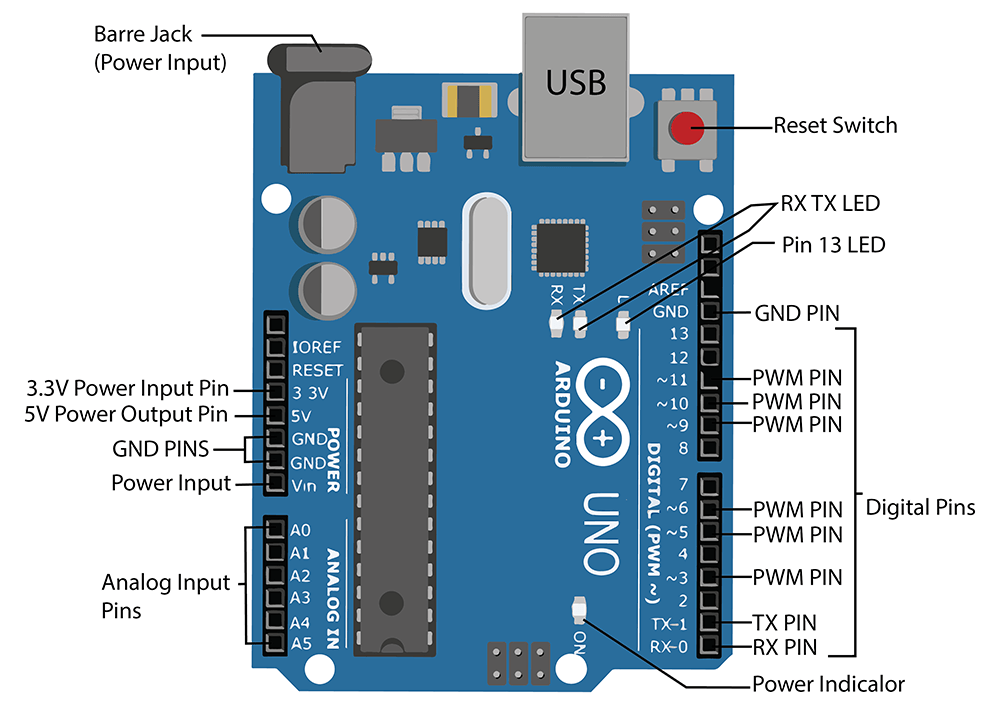
\includegraphics[width=0.5\textwidth]{foto/hardware/cph3/1.png}
    \caption{Structure of Arduino UNO}
\end{figure}
The output voltage of a GPIO pin depends on the specific microcontroller and its
operating voltage. There are some electrical constrains:
\begin{itemize}
    \item \textbf{Limited maximum current per pin}
    \item \textbf{Limited total current for all pins}
    \item \textbf{Voltage levels must be compatible with connected devices}
    \item \textbf{Use of current-limiting resistors to protect the
              microcontroller and connected components}
\end{itemize}
\subsection{Relay}
A relay is an electrically operated switch that allows a low-power signal to
control a higher power circuit. It consists of an electromagnet, a set of
contacts, and a spring mechanism. When the low-power signal energizes the
electromagnet, it creates a magnetic field that pulls the contacts together,
closing the circuit and allowing current to flow through the higher power
circuit. Relays are commonly used in applications where it is necessary to
control a high voltage or high current load with a low voltage signal, such as
in automotive systems, industrial automation, and home appliances. They provide
electrical isolation between the control circuit and the load, which can help
protect sensitive components from damage.
\begin{figure}[h]
    \centering
    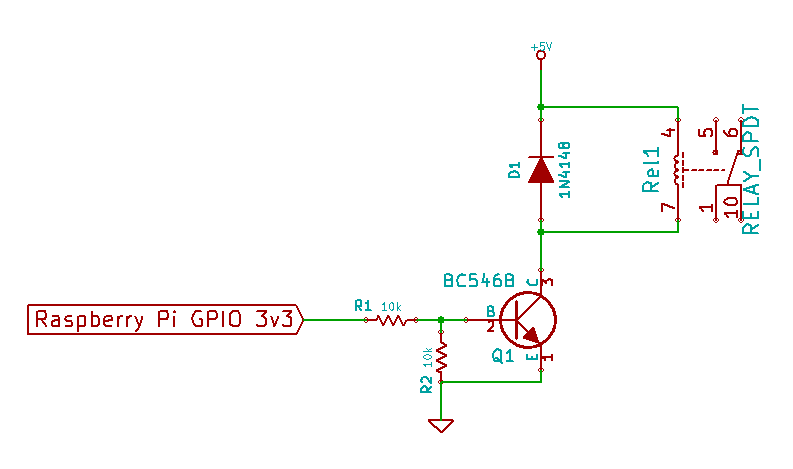
\includegraphics[width=0.45\textwidth]{foto/hardware/cph3/2.png}
    \caption{Structure of a relay}
\end{figure}
\subsection{Filtering and protection}
When controlling actuators, it is important to consider the need for filtering
and protection circuits. Filtering is necessary to remove noise and unwanted
signals that may interfere with the proper operation of the actuator.
Protection circuits are used to prevent damage to the microcontroller or other
components in case of overcurrent, overvoltage, or other abnormal conditions.
These circuits can include diodes, capacitors, resistors, and other components
that help ensure safe and reliable operation of the actuator system.
Some solutions are:
\begin{itemize}
    \item \textbf{Decoupling capacitors}: placed across the power supply lines to filter out noise and provide a
          stable voltage to the actuator.
    \item \textbf{RC/LC Low-pass Filters}:
    \item \textbf{Subnetworks}:
\end{itemize}
      